\documentclass{beamer}

\usepackage{polski}
\usepackage[utf8]{inputenc}
\usepackage{color}
\usepackage{amsfonts}	% Real

\usepackage{booktabs} % eleganckie tabelki
\usepackage{bm}		% bold math symbols


\usetheme{boxes}      % Wybór tematu wyglądu, gdy chcemy inny
%\usecolortheme{rose}   % Wybór tematu kolorystycznego, j.w.

%Konfiguracja dla pakietu hyperref:
\hypersetup{
  unicode=true,           % włączenie wyświetlania pliterek w zakładkach
%  pdfpagemode=FullScreen, % włączenie trybu pełnoekranowanego
  pdfsubject=Graph Neural Networks,      % temat prezentacji
  pdfkeywords={gnn, graph neural network, graph, classification} % slowa kluczowe
}

%% Dane do strony tytułowej
\author{Aleksy Barcz\\mgr inż. Zbigniew Szymański, II PW}
\title{Aspekty implementacyjne\\Grafowych Sieci Neuronowych}
\date{\today}
%\institute{Institute of Computer Science \\ Warsaw University of Technology}

\setbeamercovered{transparent}

\begin{document}
\frame{\titlepage}

\begin{frame}
\frametitle{Zastosowania klasyfikacji grafów}
\begin{itemize}
	\item chemia
	\item rozpoznawanie obrazów, lokalizacja twarzy
	\item przetwarzanie XML
	\item przetwarzanie języka naturalnego
	\item ranking stron WWW
\end{itemize}
\end{frame}

\begin{frame}
\frametitle{Po co nam klasyfikacja grafów?}
\begin{center}
	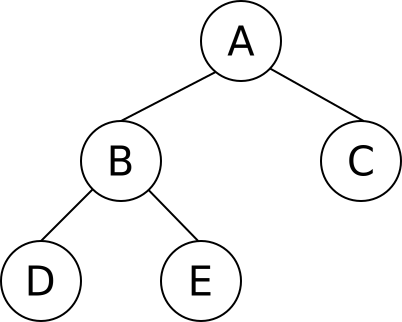
\includegraphics[scale=0.4]{img/tree}
\end{center}
Przykładowa reprezentacja wektorowa: $[A, B, C, D, E]$
\begin{itemize}
	\item problem sąsiedztwa
	\item zależności cykliczne
	\item etykiety krawędzi
\end{itemize}
\end{frame}

\begin{frame}
\frametitle{Grafowa Sieć Neuronowa (GNN, 2009)}
\begin{itemize}
	\item Klasyfikator dowolnych grafów (niepozycyjne, cykle)
	\item Oparty na sieciach neuronowych
	\item Budowanie reprezentacji jednoczesne z nauką klasyfikatora
\end{itemize}
\end{frame}

\begin{frame}
\frametitle{Zrealizowana praca}
\begin{itemize}
	\item Implementacja GNN w oparciu o publikacje
	\item Identyfikacja kluczowych parametrów
	\item Wykrycie ograniczeń modelu
\end{itemize}
\end{frame}

\begin{frame}
\frametitle{Sieć kodująca}
\begin{center}
	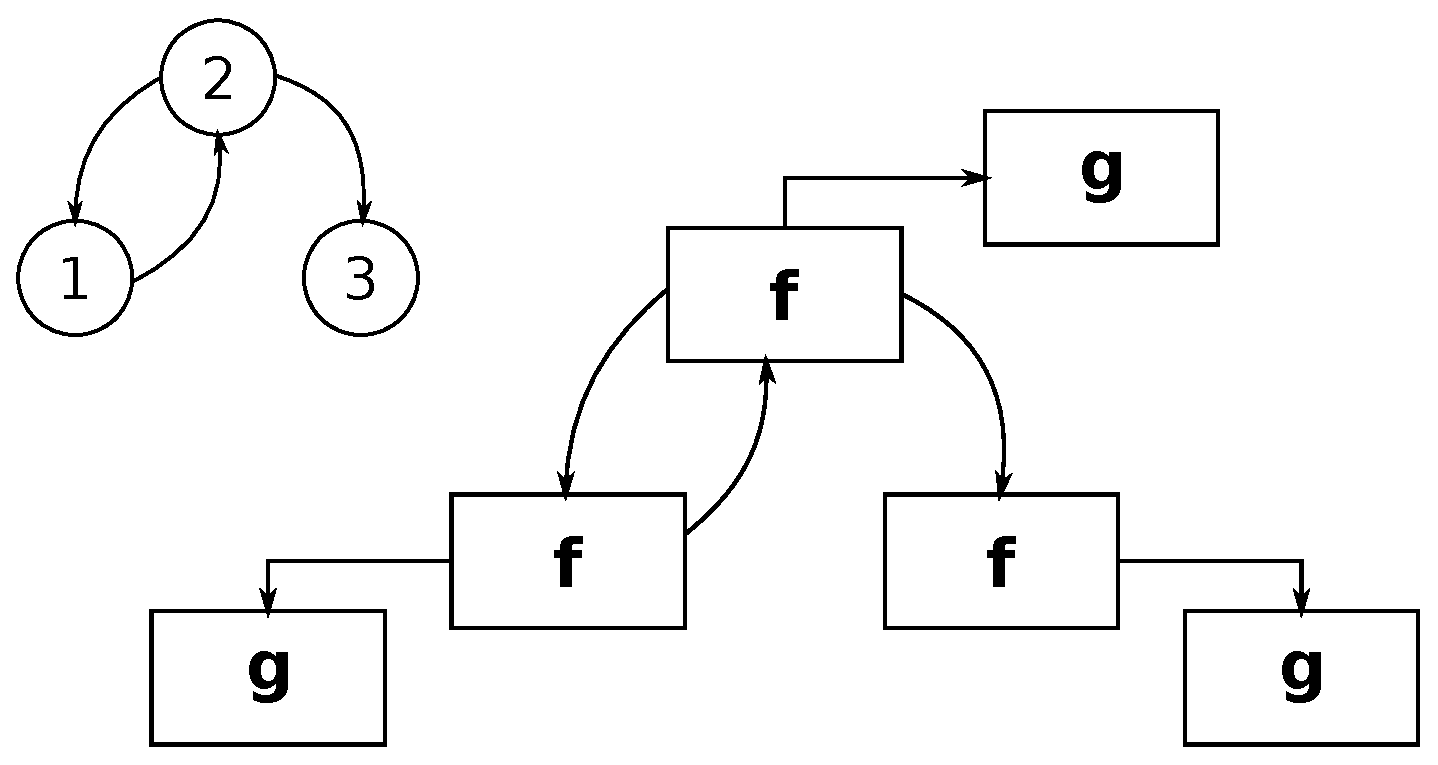
\includegraphics[scale=0.4]{img/encodinginc}
\end{center}
\begin{itemize}
	\item Dla każdego węzła budowana reprezentacja
	\item Klasyfikacja węzła na podstawie reprezentacji
	\item Wszystkie instancje $f_{\bm{w}}$ współdzielą wagi
	\item Wszystkie instancje $g_{\bm{w}}$ współdzielą wagi
\end{itemize}
\end{frame}

\begin{frame}
\frametitle{Skąd wiemy że stan osiągnie punkt stały?}
\begin{itemize}
	\item odwzorowanie zwężające (tw. Banacha)
	\item kara nakładana na wagi sieci w przypadku utraty tej właściwości
\end{itemize}
\end{frame}

\begin{frame}
\frametitle{Wpływ współczynnika kary na przebieg uczenia}
\begin{center}
	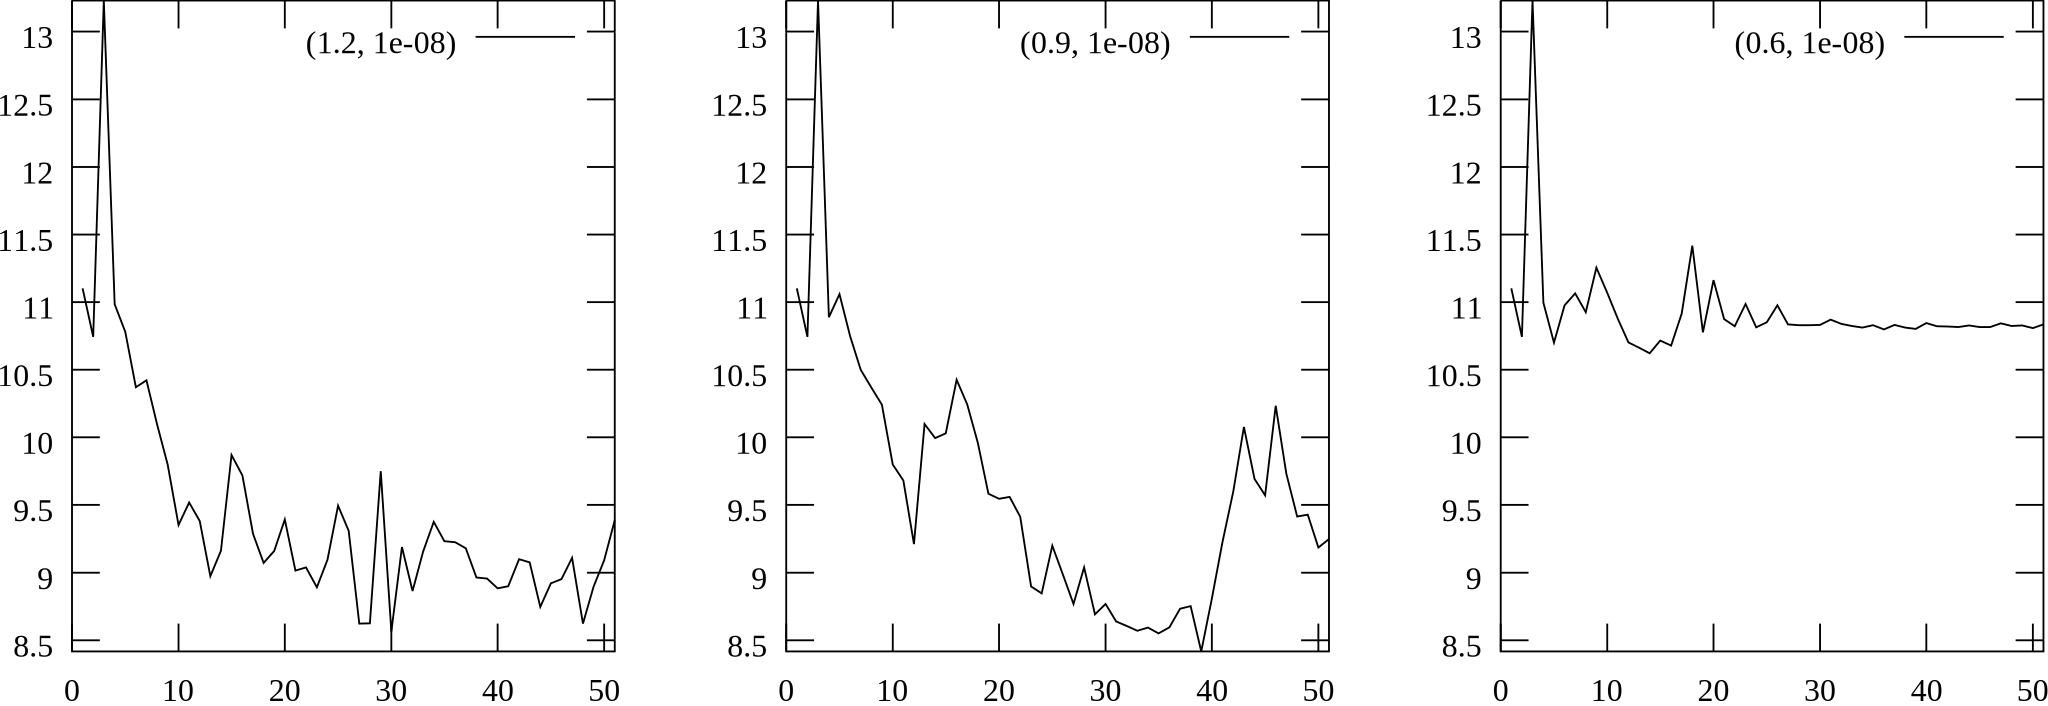
\includegraphics[scale=0.06]{img/rmse1a_clipped}
\end{center}
Istnieje minimalna wartość $\mu$ poniżej której uczenie nie zachodzi
\end{frame}

\begin{frame}
\frametitle{Oznaczanie podgrafu}
\begin{center}
	\includegraphics[scale=0.35]{img/g14s7_7clip.pdf}
\end{center}
\begin{itemize}
	\item 14 węzłów, 7 węzłów podgrafu
\end{itemize}
\end{frame}

\begin{frame}
\frametitle{Oznaczanie podgrafu - wyniki}
\setlength{\tabcolsep}{2pt}
\begin{table}[h!]
	\begin{center}
	\begin{tabular}{llll}
	\toprule
	& accuracy & precision & recall \\
	\midrule
	FNN - tr &	75\% &  68\% &  93\% \\
	FNN - tst &	74\% &  68\% &  93\% \\
	GNN - tr &	91\% &  87\% &  97\% \\
	GNN - tst &	91\% &  86\% &  97\% \\
	\bottomrule
	\end{tabular}
	\caption{Średnie wartości na zbiorze uczącym i testowym}
	\end{center}
\end{table}
\begin{itemize}
	\item FNN : najlepsza z 10ciu, 5-krotna walidacja krzyżowa
	\item GNN : losowa sieć, 5-krotna walidacja krzyżowa, 50 iteracji
\end{itemize}
\end{frame}

\begin{frame}
\frametitle{Forward - budowanie stanu}
\begin{columns}
	\begin{column}{0.66\textwidth}
		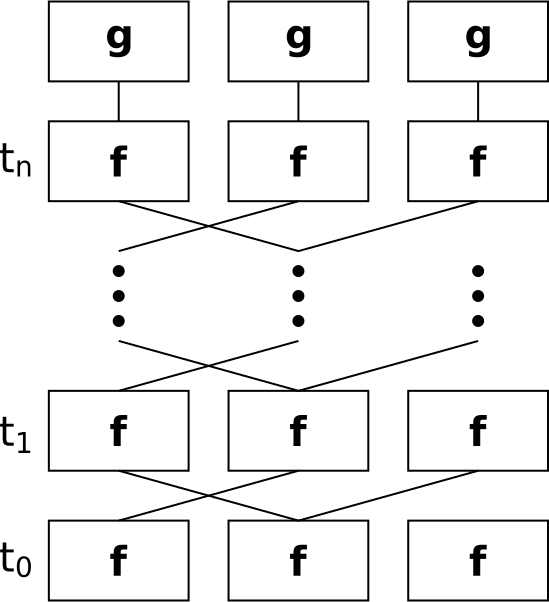
\includegraphics[scale=0.4]{img/forward}
	\end{column}
	\begin{column}{0.34\textwidth}
	\end{column}
\end{columns}
\end{frame}

\begin{frame}
\frametitle{Backward - propagacja wsteczna błędu}
\begin{columns}
	\begin{column}{0.66\textwidth}
		\includegraphics[scale=0.4]{img/backward}
	\end{column}
	\begin{column}{0.34\textwidth}
	\end{column}
\end{columns}
\end{frame}

\begin{frame}
\frametitle{Poprawny przebieg uczenia}
\begin{center}
	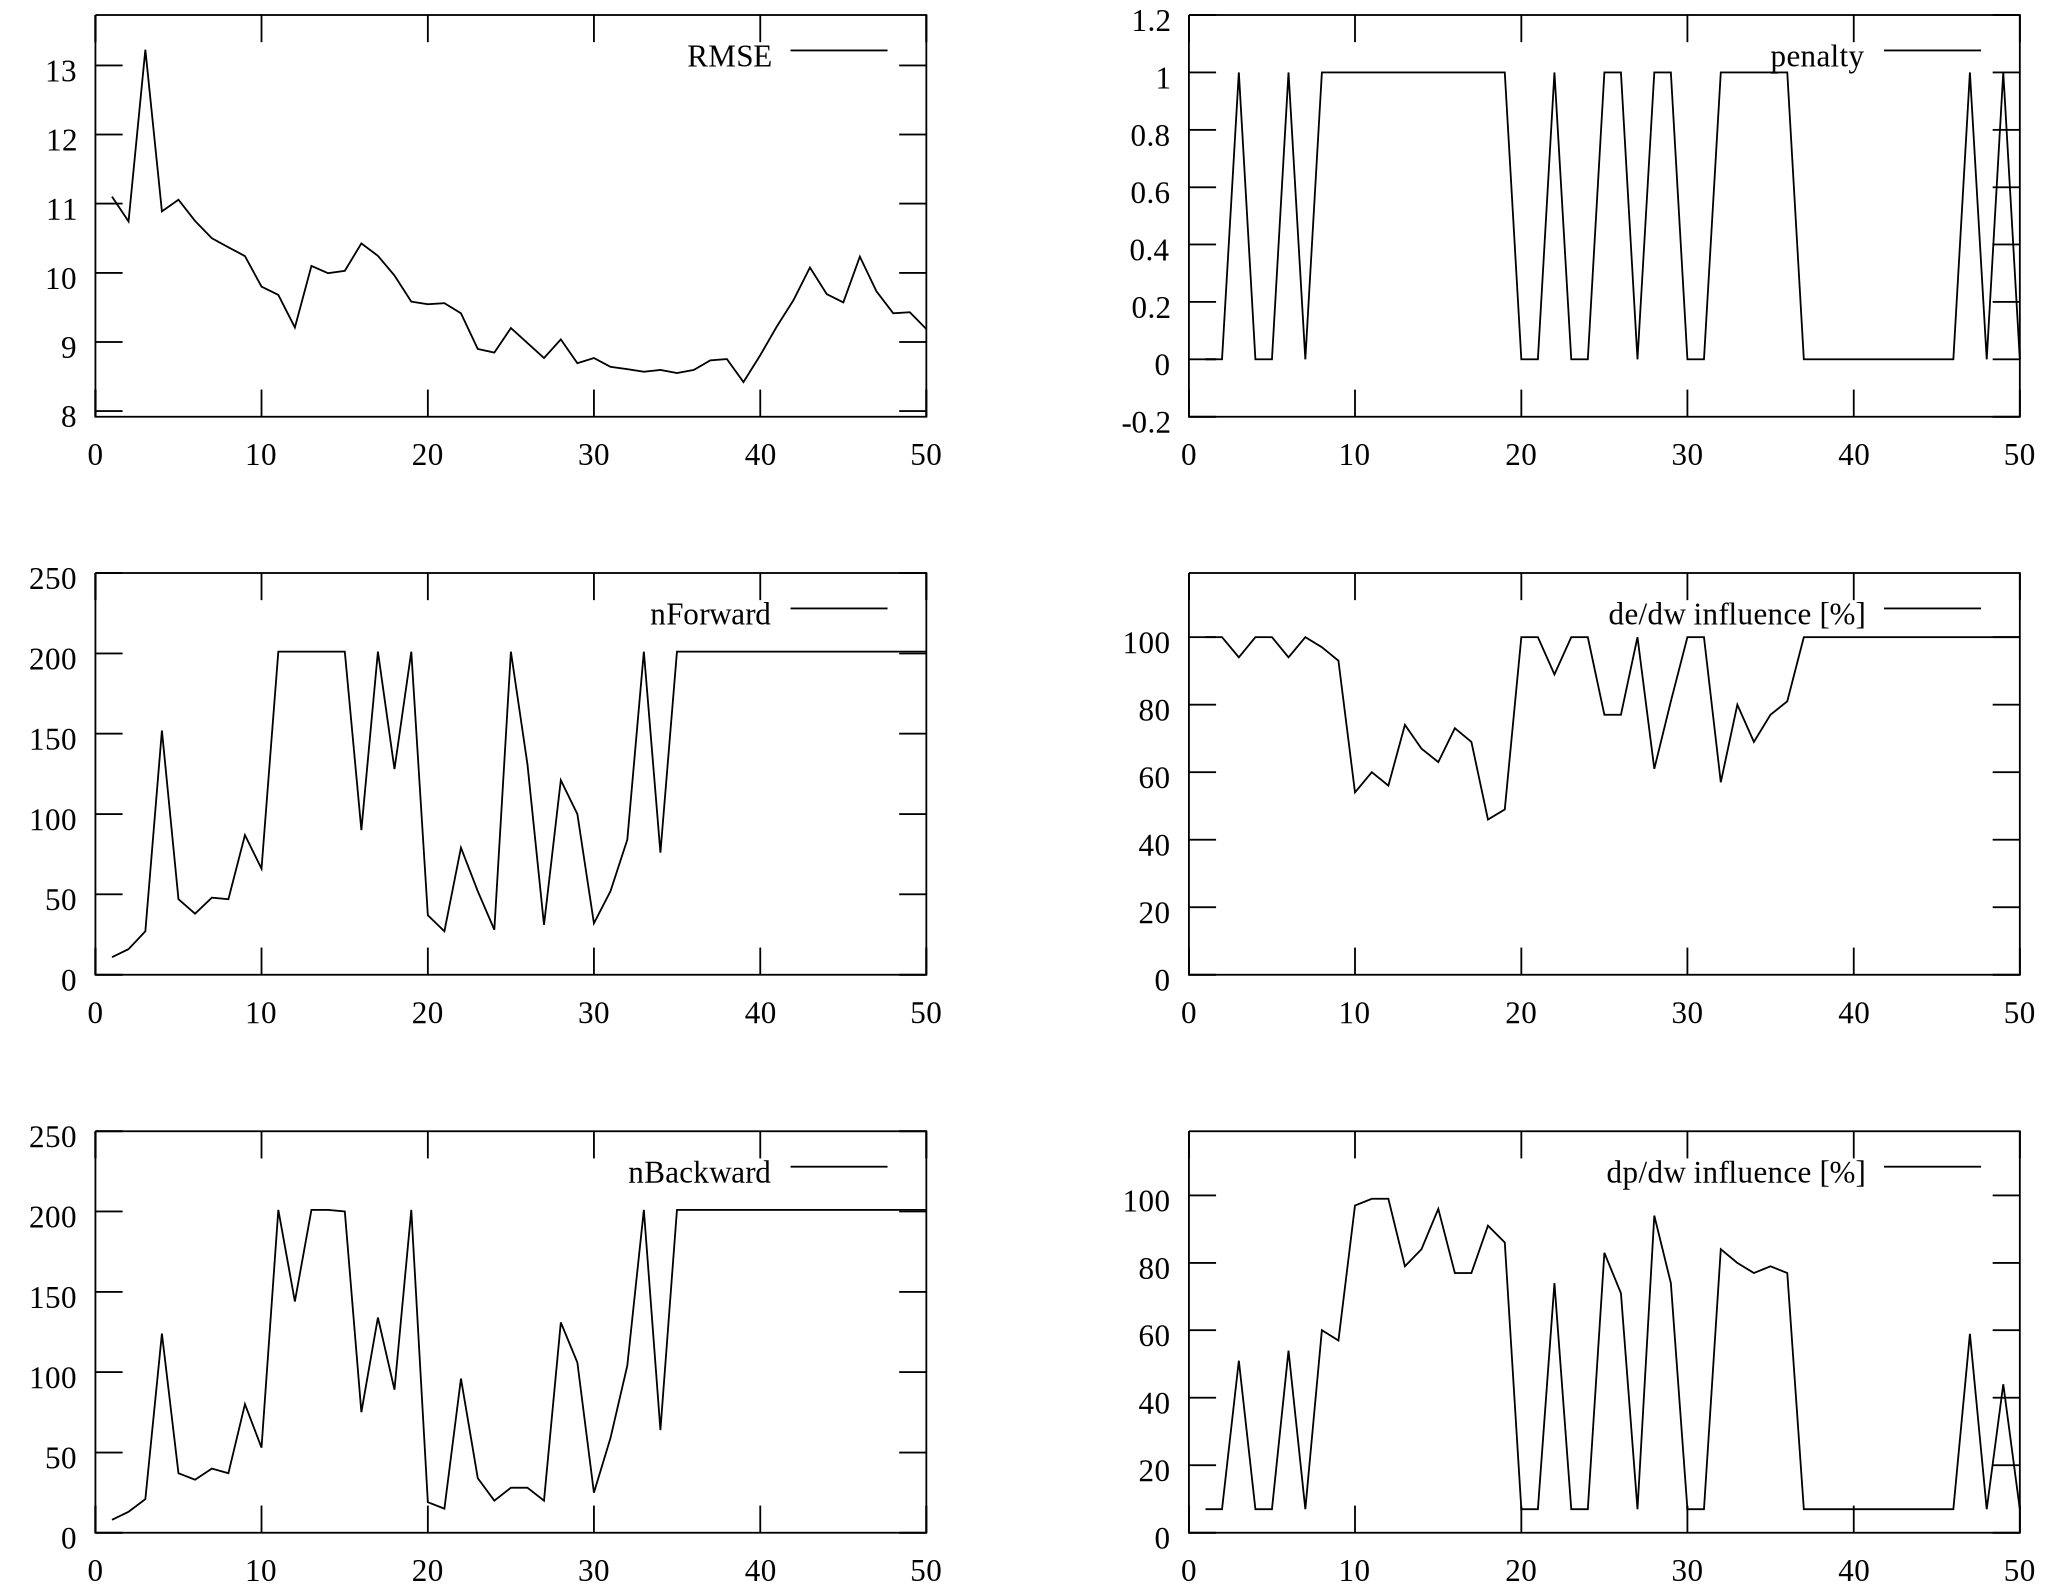
\includegraphics[scale=0.06]{img/gnn1_2}
\end{center}
\end{frame}

\begin{frame}
\frametitle{Zaburzenie procesu uczenia}
\begin{center}
	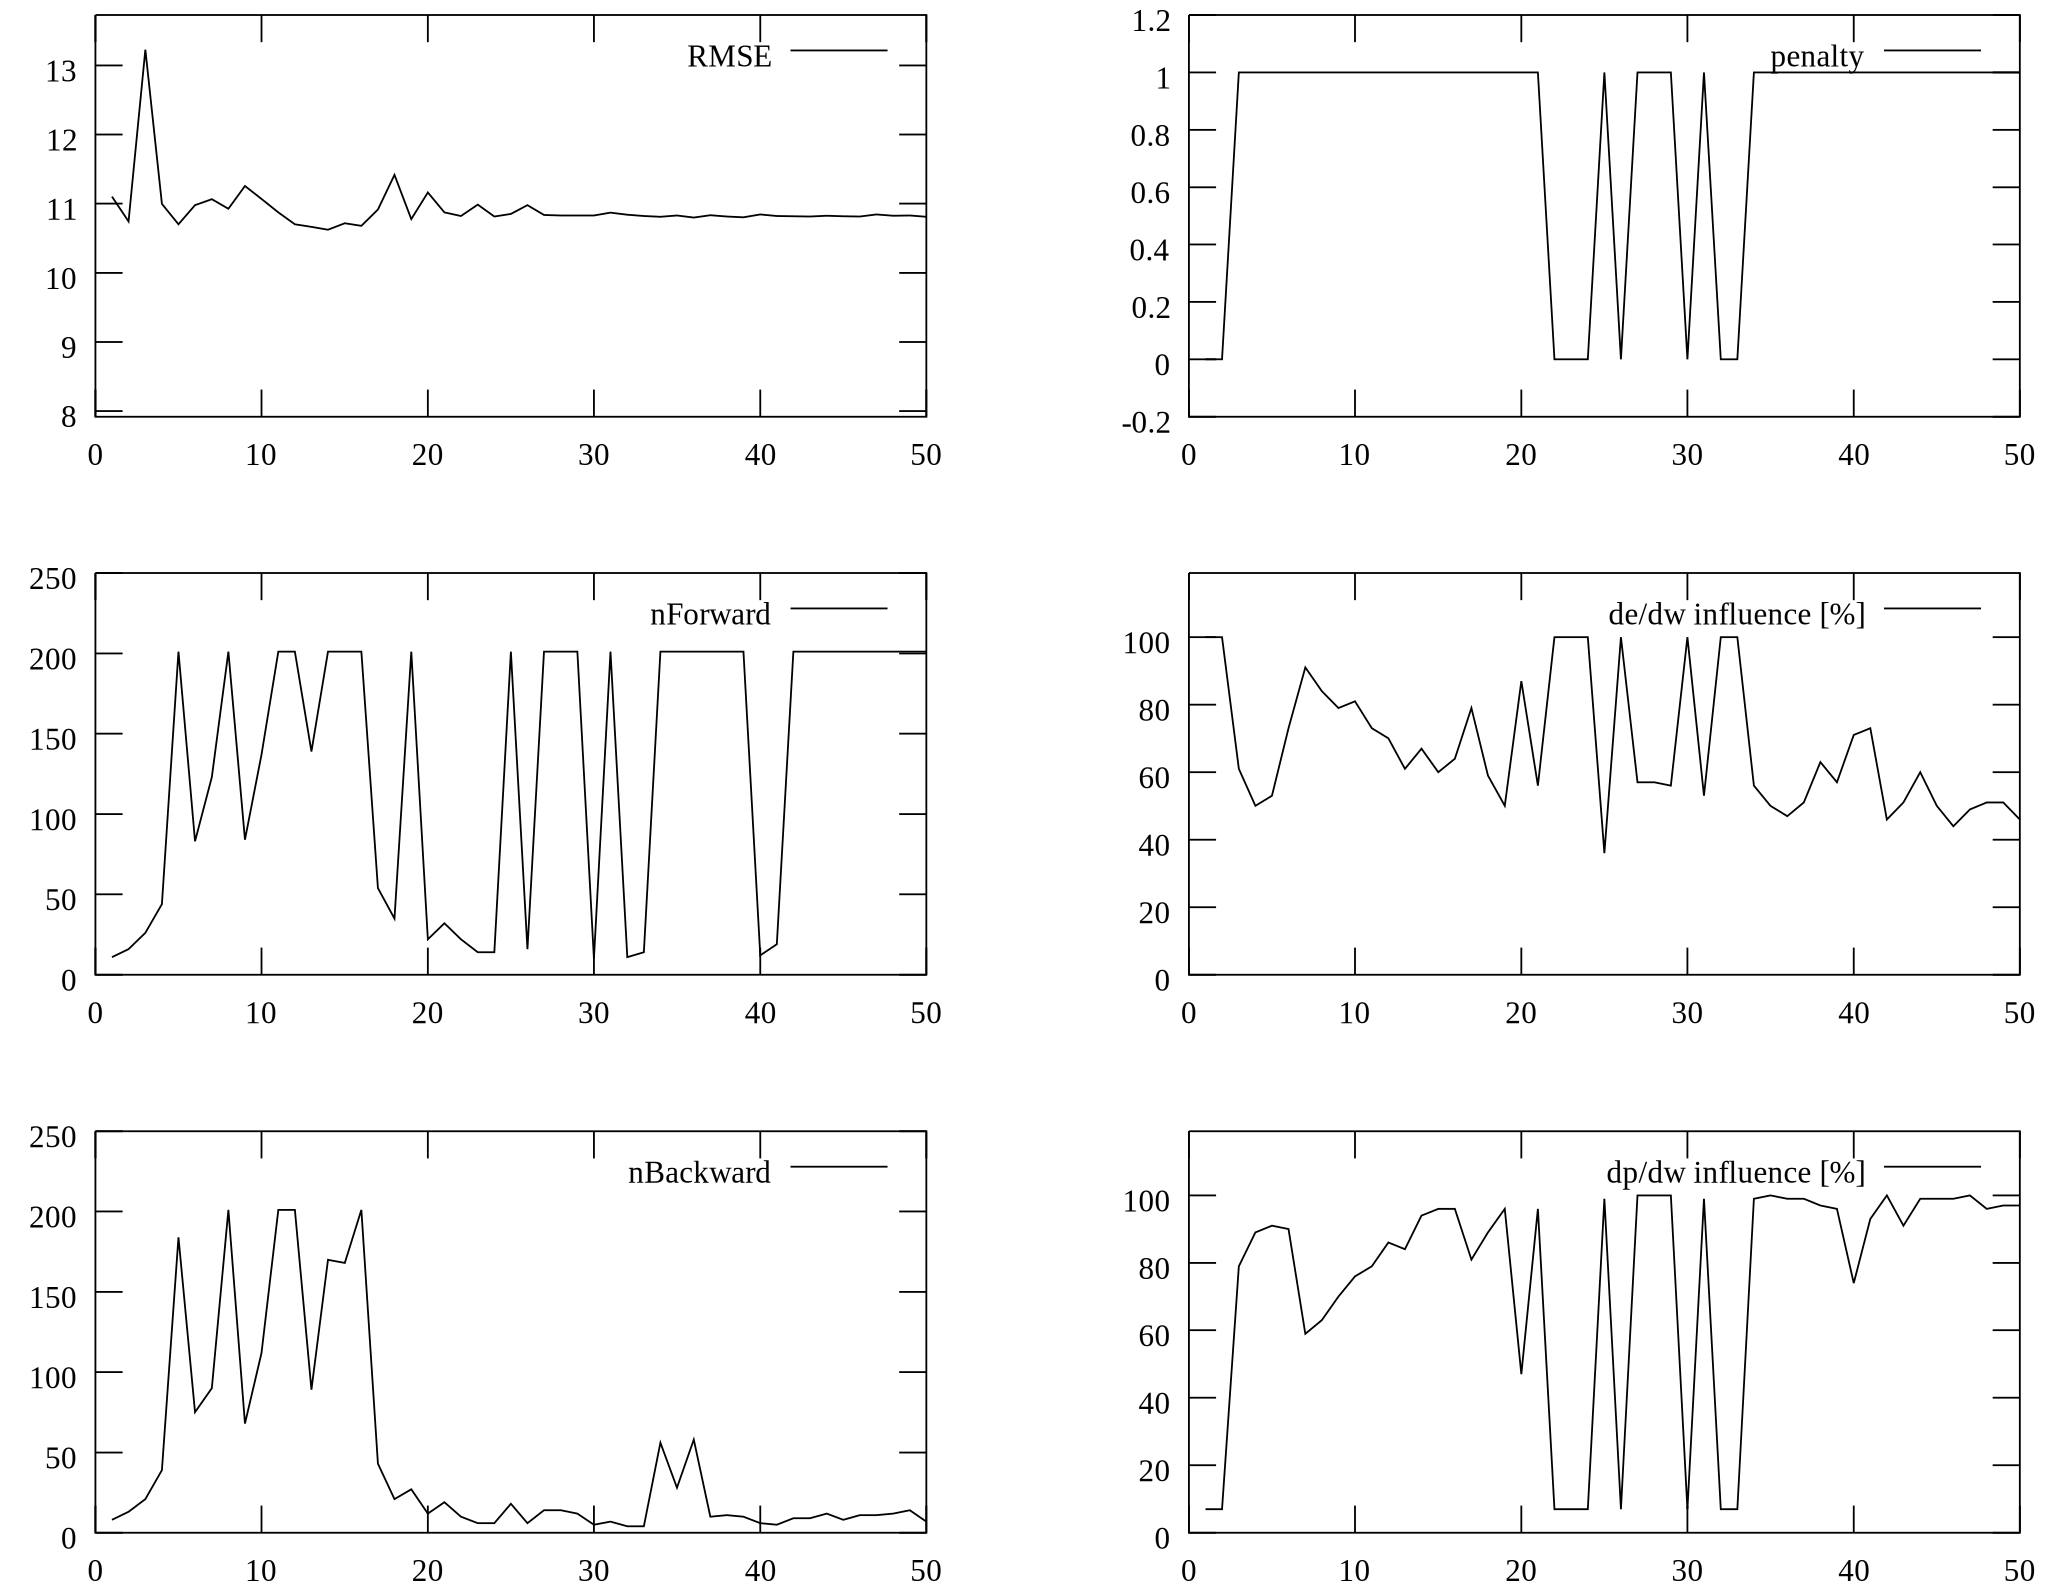
\includegraphics[scale=0.06]{img/gnn1_3}
\end{center}
\end{frame}

\end{document}
